\chapter{Conclusion and Future work} During this thesis, we have proposed a promising system to recognize hand gestures based on skeletal points tracking using depth camera. This system is built for the purpose of human-robot interaction (HRI) with the humanoid robot named as NAO. We have validated this approach by training the system with five static gestures and obtained results as shown in the section \ref{ch:result}.

We have partitioned our goal into 4 modules and reached the goal by implementing them in a decoupled environment, and finally, integrated all of them into one system. We have shown that proposed approach is sufficiently robust and flexible to deal with static hand gestures. 

Human-Robot Interaction (HRI) module deals with integrating the depth camera into the robot and processing the depth information to track the skeletal points of the user, and finally send them via network to the Brain module. Brain module supports the core functionalities of this system by receiving the skeletal point information of the user, and recording them as training data in the training mode or computing the prediction results in the prediction mode. Control Center (CC) module plays vital role in visualizing these interactions, therefore, it is considered as the eye of the system. Finally, Command module comprehends the predicted gesture and translating them to a robotic Motion or Speech or Gesture itself.

Finally, we have carried out several experiments and provided the results which illustrate the robustness of the system. Furthermore, we have done evaluations on the test data and plotted them on graph to visually understand the performance of the system. 

\section{Discussion} 
We have faced issues in implementing few contemplated solutions due to various limitations. Following section discusses about few experimental designs which are conceived during thesis.

\subsection*{Everything On-Board} First experiment design is conceived in a way that depth camera, skeletal joint tracking, gesture recognition infrastructure and robot motion will be embedded into the on-board computer of NAO. However, gesture recognition infrastructure is composed of computationally intensive machine learning processes and along with skeletal joint tracking by NiTE had pushed NAO to full CPU load consistently \cite{17}.

\subsection*{Extending NAO with Single Board Computer} In order to overcome the computational limitation of NAO, another experimental design is contemplated that the robot will be extended as shown in the figure \ref{fg:nao:bag} with a powerful Single Board Computer such as pcDuino or RaspberryPi. However, Asus Xtions higher power consumption of 2.5 Watts with weight of 250 grams, pcDuinos power consumption of 2A at 5VDC with weight of 100 grams and additional weight by 3D printed mounts, heat sinks and wires will make NAO heavier and ultimately result in poor motion performances and higher power consumption. 

\begin{figure}
	[h] \centering 
	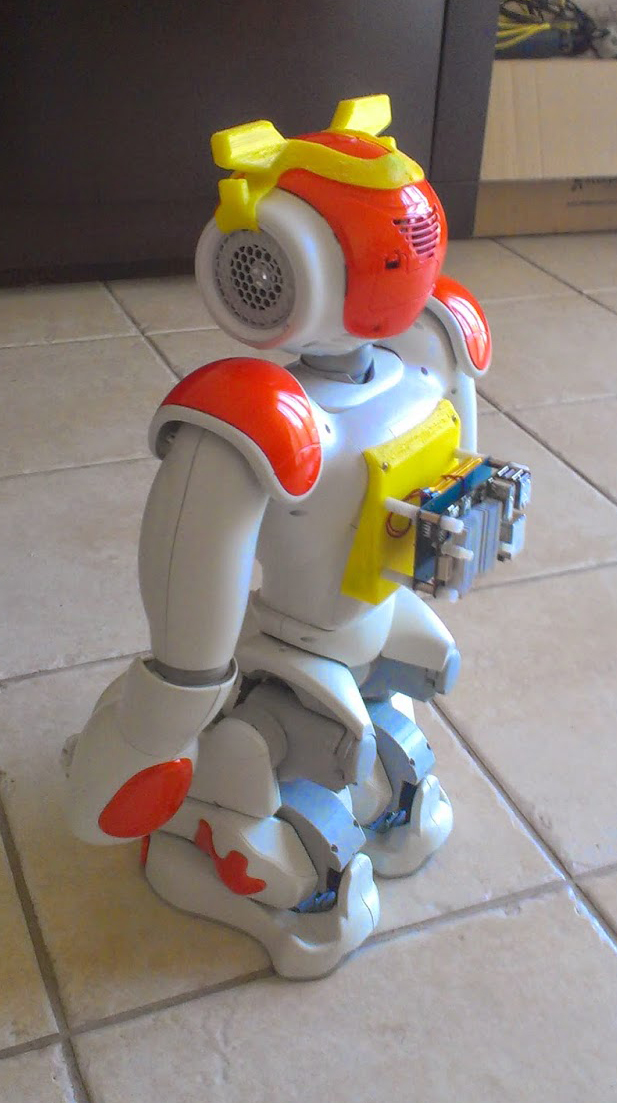
\includegraphics[height=7cm]{figures/content/nao-bag.jpg} \caption{3D printed mount to extend NAO with an external Single Board Computer. \cite{19} } \label{fg:nao:bag} 
\end{figure}


\subsection*{Everything Off-Board} This experimental design pushes all the components to an off-board computer that could be a PC connected with depth camera at a fixed location. User will gesticulate in front of the camera and all processing will be done on PC. Finally predicted gesture will be transformed into a motion and voice, and it will be sent to NAO via Aldebaran proxies using WLAN. This design completely decouples the robot from other components and degrades the natural interaction between human and the robot. However, this design will suit for other applications such as indoor navigation and localization of NAO \cite{20}.

\section{Future Work} The proposed design for gesture recognition based on skeletal points tracking using depth camera can be improved in several ways. In this section, we overview the future work by discussing the limitations of the proposed methods and proposing the alternatives.
\begin{itemize}
	\item \textbf{Networking} : 4 modules of this system is connected via several networking components such as UDP Server-Client, Websocket Server-Client and NAOqi proxy. Server-Client networking topology involving different communication protocol is a big limitation, since every module have implemented their own server or client functionalities of UDP or WebSocket. Furthermore, data is serialized as JSON strings and must be parsed at the receiver side to extract the data. Hence, we propose Open Sound Control (OSC) protocol that covers all these requirements in one framework with distributed networking topology.
	
	\item \textbf{Graphical User Interface} : Since the components of this system are modularized and developed independently, the development environment varies with each other. Even though WebGL is easier and flexible graphics library, it takes a lot of processing power as it runs on the browser. Instead of using several programming languages, the system could be implemented with C++ GUI using QT or Microsoft Visual C++ and OpenGL. We propose to integrate the existing code into such framework to build this system as standalone application. 
	
	\item \textbf{Skeleton Joints} : Due to computational limitations of NAO, in this thesis, we have used only hand joints of the user to train and classify the gestures. Classification based on positions of only hand joints does not allow us to train many gestures because the gesture model will higher rate of confusion. For instance, in Cartesian coordinates "Hands Up" gesture trained at different distances from the sensor will be confused with "Hands Wide". Therefore, we propose to make use of other skeleton joints such as shoulder and arm to calculate the orientation of hand in polar coordinates.
	
	\item \textbf{Computational Limitations of NAO} : In this thesis, HRI module is deployed to general purpose computer of NAO. HRI module is responsible for tracking the hand or full skeleton joints with the help of NiTE framework. NiTE uses computationally intensive algorithms and causes higher CPU utilization of NAO. Therefore, we propose to transmit the depth information from OpenNI device completely to NiTE application on an off-board computer. This could be achieved by using Robot Operating System (ROS) framework that already has a solution to transmit depth information via network.
	
	\item \textbf{Temporal Gestures} : During this thesis, we have trained our system to recognize only static gestures which imply an action such as traffic police signals. However, human natural interaction is comprised of many more sophisticated dynamic gestures. Therefore, we propose to extend this system with Dynamic Time Warping classifier of GRT with Time-Series-Classification data to recognize temporal gestures. 
\end{itemize}


